\documentclass{beamer}
\usepackage{fontspec}
\usepackage{polyglossia}
\usepackage{multicol}
\usepackage{luabidi}
\usepackage{xcolor}
\usepackage{graphicx}
\usepackage{float}
\usepackage{wrapfig}

\setmainlanguage{arabic}
\setotherlanguage{english}
\newfontfamily\arabicfont[Script=Arabic, Scale=1.0]{Amiri}
\setsansfont{Amiri} %(c) You have to put this extra command with {beamer} for the arabic language.
\newfontfamily\englishfont{Latin Modern Roman}
% \setmainlanguage[numerals=western]{arabic} %(c) For using Arabic numbers instead of the Indian.
\newcommand{\ar}{\textarabic}
\newcommand{\en}{\textenglish}


% \usetheme{Warsaw}
% \usetheme[progressbar=frametitle]{metropolis} %(c) that didn't work with the arabic so I used this:
% \usetheme{metropolis}
% \setbeamertemplate{frame numbering}[fraction]%(c) is not good with the arabic.
% \useoutertheme{metropolis}
% \useinnertheme{metropolis}
% \usefonttheme{metropolis}
% \usecolortheme{spruce}
% \setbeamercolor{background canvas}{bg=white}

% \definecolor{ferngreen}{rgb}{0.31, 0.47, 0.26} %(c) I defined this color for the theme
% \usecolortheme[named=ferngreen]{structure}
% \definecolor{mytextgreen}{rgb}{0.0, 0.65, 0.31} %(c) I defined this color for the text below 

% \setbeamercovered{transparent=15} %(c) It applies only on \onslide command.

% \title{تقرير زيارة ميدانية إلى محطة تحويل \en{A1} \textendash مدينة حلب}
% \author{إعداد الطالب : محمد علي قطان \en{207047}}
% \institute{
%   مقرر: تصميم نظم القدرة 2\\[2pt]
%   بإشراف الدكتور: خالد شيخ حمود\\[2pt]
%   والمهندسة: بيان عقاد
%   }
% \date{\small تاريخ الزيارة : \en{15} كانون الأول/ديسمبر \en{2025}}

% \setbeamertemplate{headline}{
%   \begin{beamercolorbox}[wd=\paperwidth,ht=2.2cm,dp=0.8cm]{}
%   \begin{picture}(0,0)
%   \put(270,-25){
\includegraphics[width=2.3cm]{logo.png}}
%   \end{picture}
%   \begin{picture}(0,0)
%     \put(30,20){%
%         \parbox[t]{5cm}{% %(c) this command determines the width of the content (without triping). 
%         \raggedright
%         \normalsize %(c) Some commands change the size of there content; this command prevents the size change form being applied.
%         \fontsize{8pt}{11pt}\selectfont 
%         \hspace{21pt}\textbf{جامعة حلب}\\
%         \hspace{-11pt}كلية الهندسة الكهربائية والإلكترونية\\
%         قسم نظم القدرة الكهربائية
%         }
%       }
%     \end{picture}
%   \end{beamercolorbox}
% }


\begin{document}
%(c) In Beamer we create frames to hold all of our information, a frame can contain a single slide in your slide presentation, or it can actually contians multiple slides 

% \begin{frame}
%   \vspace{-1.6cm}
%   \titlepage
% \end{frame}

% \setbeamertemplate{headline}{} %(c) To remove the header from the next slides.

% \begin{frame}{التعريف بمحطة تحويل حلب وهويتها الفنية}
%     % \fontsize{9pt}{11pt}\selectfont %(c) To control the font size (9pt) and the space between the lines(or the baseline skip) (12pt).
%     \begin{columns}[onlytextwidth]
%       \column{0.35\textwidth}
%     \textbf{نبذة تاريخية ونظام التصميم:}\\[5pt]
%     تُعد هذه المحطة من أقدم وأهم المحطات في شبكة مدينة حلب، وهي مصممة وفق النظام الفرنسي ويعود تاريخ إنشائها إلى عام \en{1968}.\\[5pt]
%     \column{0.5\textwidth}
%     \vspace{20pt}
%     \centering
%     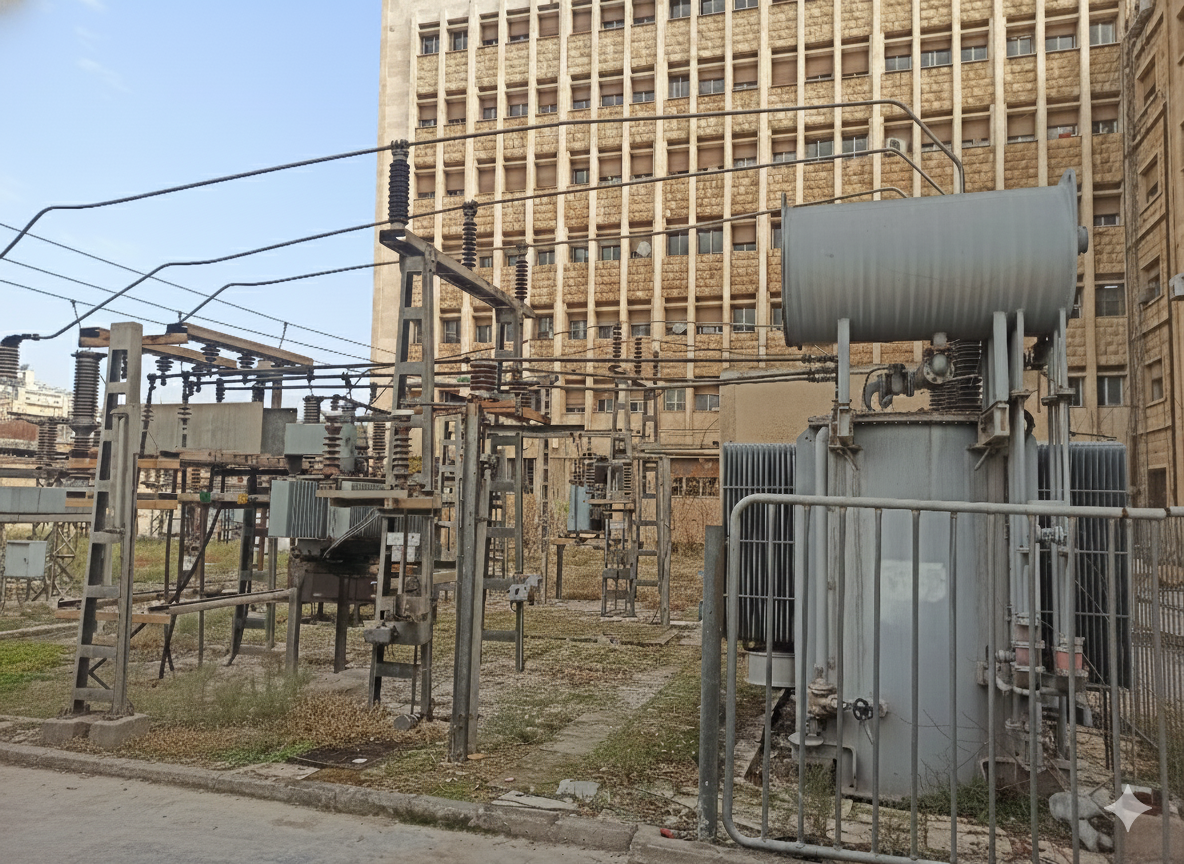
\includegraphics[width=1\linewidth]{Ph1.png}
%     {\footnotesize\scriptsize محطة التحول \en{A1} ذات الجهد المتوسط \textendash\,مدينة حلب}
%     \end{columns}
%     \textbf{الدور الاستراتيجي:}\\[5pt]
%     تعمل المحطة كمحطة توزيع رئيسية \en{(Sub-transmission)}؛ حيث تستقبل الجهود العالية جداً وتقوم بتحويلها وتوزيعها لتغذية أحياء سكنية وتجارية حيوية في حلب، مثل: الجميلية، الأشرفية، السليمانية، التلل، والعزيزية.\\
% \end{frame}

% \begin{frame}{التعريف بمحطة تحويل حلب وهويتها الفنية}
%   \textbf{مستويات الجهد الكهربائي في المحطة:}
%   تتعامل المحطة مع منظومة متكاملة من الجهود تشمل:
%   \begin{enumerate}
%     \fontsize{10pt}{12pt}\selectfont
%     \item \textbf{جهد \en{230} كيلو فولت:} الخطوط القادمة من محطات التوليد الحرارية.
%     \item \textbf{جهد \en{66} كيلو فولت:} جهد النقل الثانوي وتوزيع الطاقة بين المحطات.
%     \item \textbf{جهد \en{20} كيلو فولت:} الجهد الذي يتم توزيعه على مراكز التحويل في الأحياء السكنية.
%     \item \textbf{جهد \en{6} كيلو فولت:} نظام قديم كان مستخدماً في المحطة (النظام الفرنسي)، ولا يزال موجوداً بشكل محدود جداً لبعض المنشآت الخاصة مثل محطات المياه أو الإسمنت.
%   \end{enumerate}
  
%   \textbf{طراز المحطة المعماري والتقني:} تضم المحطة قسمين رئيسيين:
%   \begin{itemize}
%     \fontsize{10pt}{12pt}\selectfont
%         \item \textbf{الساحة الخارجية \en{(Switchyard)}:} وهي المحطة "الهوائية" التي تعتمد على الهواء الطبيعي كوسط عازل بين الفازات.
%         \item \textbf{القسم المعزول بالغاز \en{(GIS)}:} وهو القسم الحديث "المغلق" الذي يستخدم غاز السداسي فلوريد الكبريت \en{(SF6)} كعازل لتوفير المساحة وزيادة الأمان.
%   \end{itemize}
% \end{frame}

\begin{frame}{ساحة التوزيع والمعدات الخارجية }
    \fontsize{10pt}{12pt}\selectfont
   تُسمى الساحة الخارجية بهذا الاسم لأنها محطة "هوائية"، حيث يُستخدم الهواء الطبيعي كوسط عازل بين الفازات والمعدات، وتُصمم المسافات بين الناقلات بناءً على مستوى الجهد (مثلاً جهد \en{66} كيلو فولت يتطلب مسافة عازلة تبلغ حوالي \en{16} سم).

  \vspace{10pt}
  \begin{columns}[onlytextwidth]
    \begin{column}{0.4\textwidth}
      \textbf{خطوط الدخول :} تستقبل الساحة خطوطاً بجهد \en{66} كيلو فولت قادمة من محطات أخرى مثل (محطة الشركـة ومحطة الجامعة)، 
      أو خطوطاً بجهد \en{230} كيلو فولت قادمة من محطات التوليد الحرارية (مثل خط الصاخور وحلب الجديدة).
    \end{column}
      \begin{column}{0.6\textwidth}
      \centering
      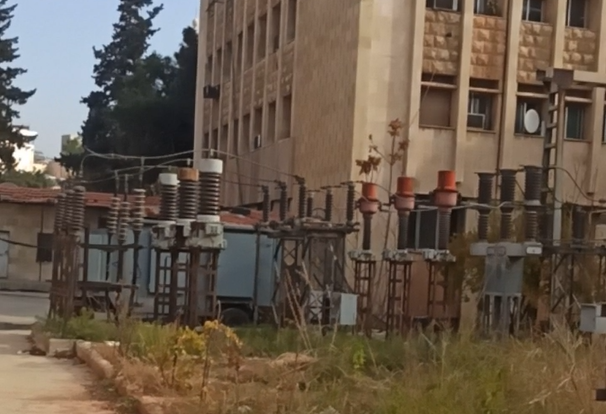
\includegraphics[width=0.9\linewidth]{Ph2.png}\\
      {\footnotesize\scriptsize مكان ربط خطوط \en{66} كيلو فولت القادمة من محطة الجامعة}
    \end{column}
  \end{columns}
\end{frame}

\begin{frame}{ساحة التوزيع والمعدات الخارجية }
  \textbf{أجهزة القياس والتحويل :}\\[15pt]
  \begin{itemize}
    \begin{columns}[onlytextwidth]
      \begin{column}{0.4\textwidth}
      \item \textbf{محولات التوتر \en{(VT)}:} وظيفتها قياس الجهد على الخطوط وتحويله لقيم صغيرة تناسب أجهزة القياس لتبين قيمة كل فاز \en{(R, S, T)}.\\[10pt]
      \item \textbf{محولات التيار \en{(CT)}:} تظهر في الساحة باللون الأحمر، ووظيفتها تحديد نسب التيار المارة في الخطوط لأغراض الحماية والقياس.\\
      \end{column}
        \hspace{0.2cm}
      \begin{column}{0.6\textwidth}
        \begin{columns}
          \begin{column}{0.48\textwidth}
            \centering
            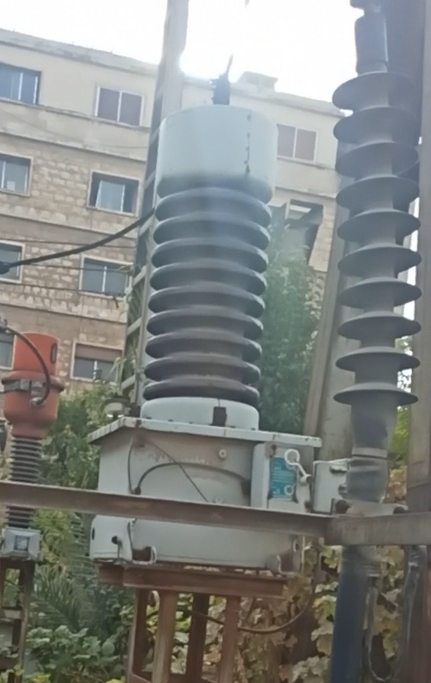
\includegraphics[width=3.2cm, height=4.5cm]{Ph3.png}\\
            {\footnotesize\scriptsize محول توتر \en{VT}}
          \end{column}
            \hspace{-0.9cm}
          \begin{column}{0.48\textwidth}
            \centering
            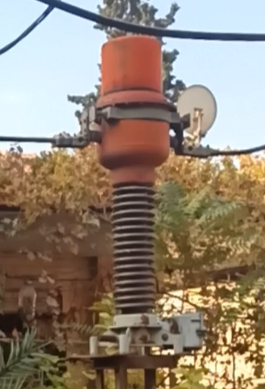
\includegraphics[width=3.2cm, height=4.5cm]{Ph4.png}\\
            {\footnotesize\scriptsize محول تيار \en{CT}}
          \end{column}
        \end{columns}
      \end{column}
    \end{columns}
  \end{itemize}
\end{frame}

\begin{frame}{ساحة التوزيع والمعدات الخارجية }
  \textbf{معدات الفصل والوصل:}\\[5pt]
  \begin{columns}
      \fontsize{10pt}{12pt}\selectfont
    \begin{column}{0.5\textwidth}
      \begin{itemize}
          \item \textbf{القواطع الآلية :} وهي قواطع تعمل بغاز \en{SF6} (سداسي فلوريد الكبريت) لإطفاء القوس الكهربائي، وتُستخدم لفصل الخطوط أو المحولات آلياً عند حدوث أعطال.\\[5pt]
          \item \textbf{السكاكين :} تُستخدم للفصل الميكانيكي الظاهر للعين لتأمين مسافة أمان أثناء الصيانة، وتتحرك يمين يسار لفتح الدارة.\\
      \end{itemize}
    \end{column}
        \hspace{-1.4cm} %(c) this thing is the most bueatiful thing in the world.
    \begin{column}{0.5\textwidth}
        \vspace{-0.65cm}{% %(c) This for rising the pictures only.
      \begin{columns}
        \begin{column}{0.5\textwidth}
          \centering
          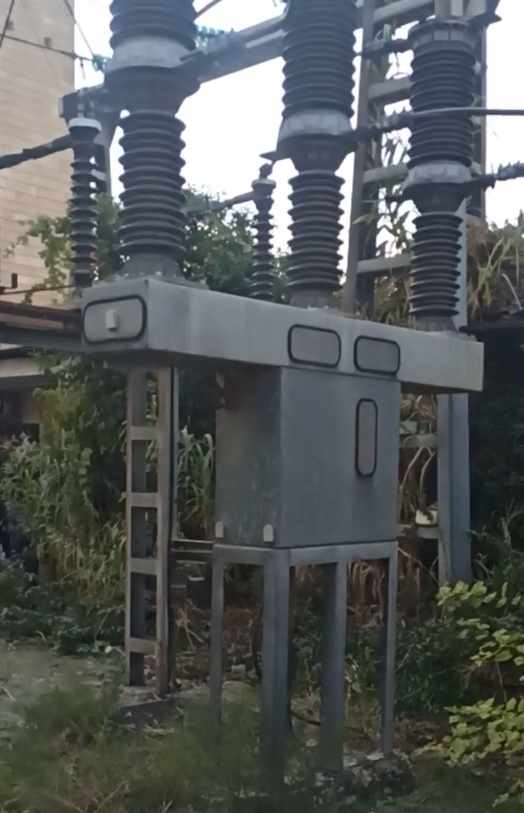
\includegraphics[width=3cm, height=4.2cm]{Ph5.png}\\
          {\footnotesize\scriptsize قاطع آلي }
        \end{column}
          \hspace{-0.5cm}
        \begin{column}{0.5\textwidth}
          \centering
          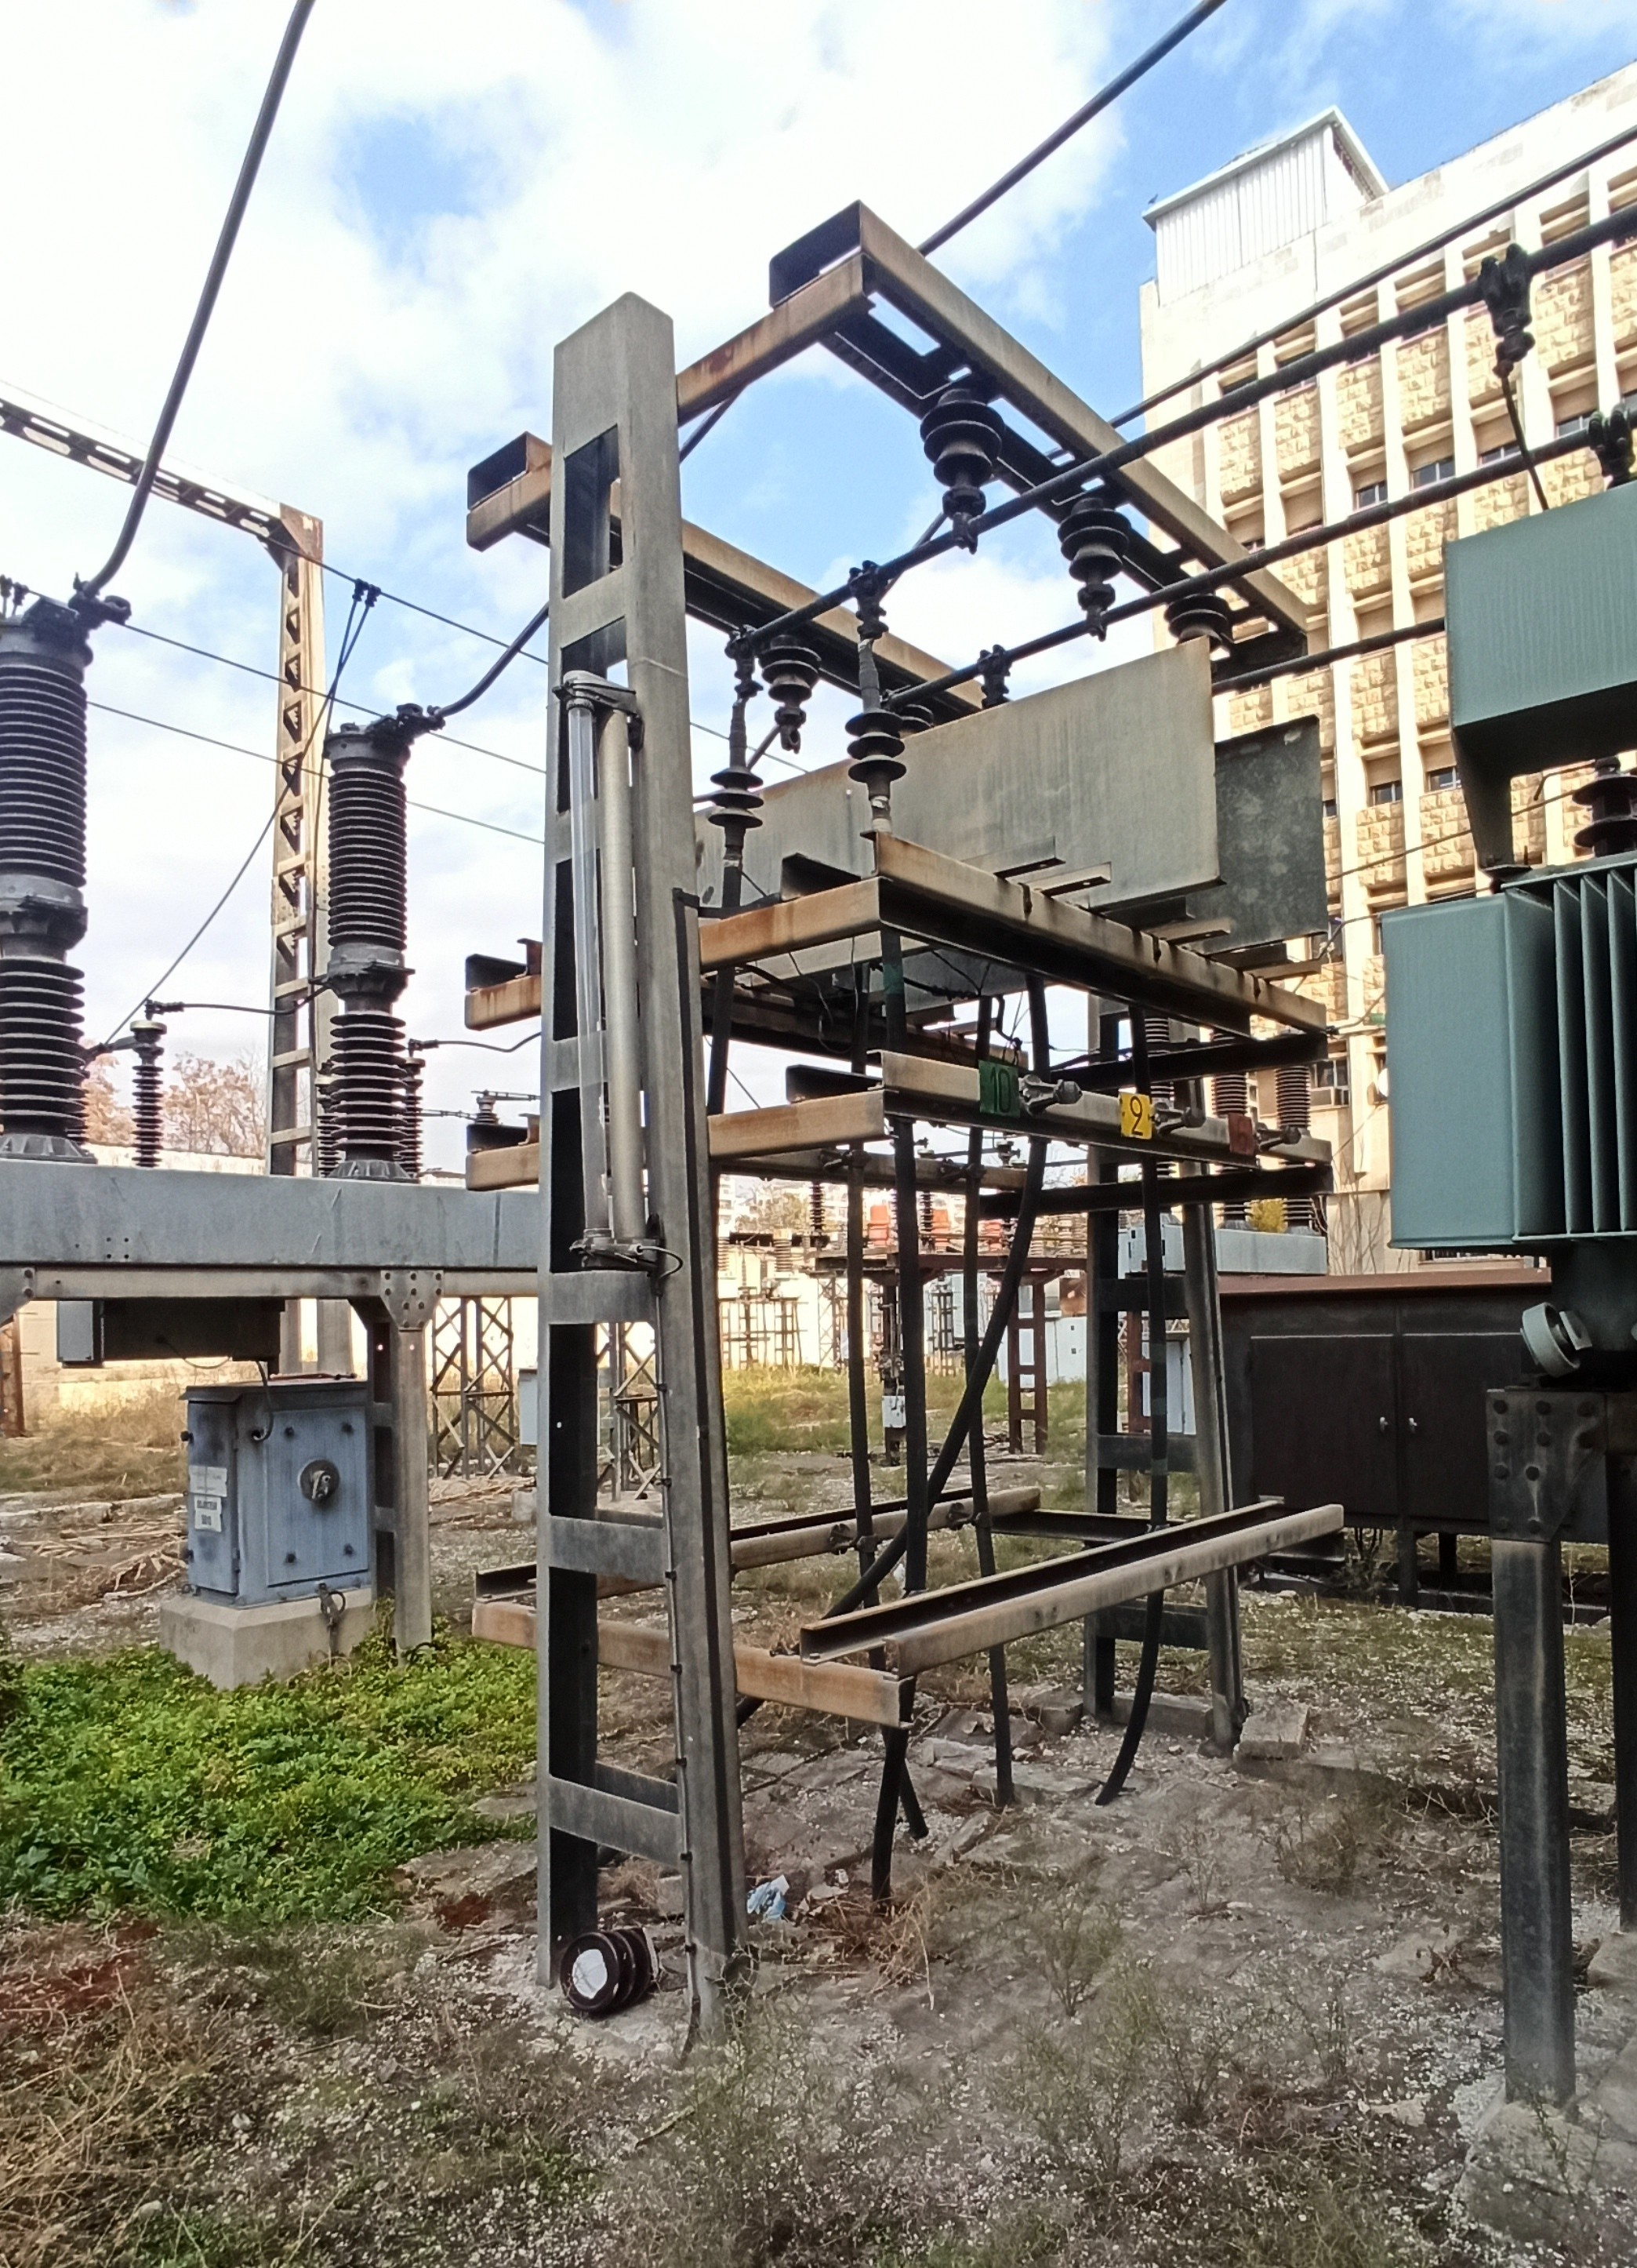
\includegraphics[width=3cm, height=4.2cm]{Ph6.jpg}\\
          {\footnotesize\scriptsize قاطع فصل هوائي}
        \end{column}
      \end{columns}}
    \end{column}
  \end{columns}
\end{frame}

\begin{frame}{المحول الرئيسي (القلب النابض)}
    \fontsize{10pt}{12pt}\selectfont
    % \metroset{block=fill}
    % \begin{block}{المحول الرئيسي}
      \begin{columns}
      \begin{column}{0.4\textwidth}
      هو العنصر المركزي الذي يقوم بالوظيفة الأساسية للمحطة، وهي تحول الطاقة الكهربائية من جهد عالٍ (\en{66} كيلوفولت) إلى جهد مناسب لشبكة التوزيع (\en{20} كيلوفولت)، التوصيل فيه يكون نجمي للملف الابتدائي ومثلثي للثانوي. 
    \end{column}
  
    \hspace{-1.2cm}
  
    \begin{column}{0.4\textwidth}
      \vspace{10pt}
      \centering
      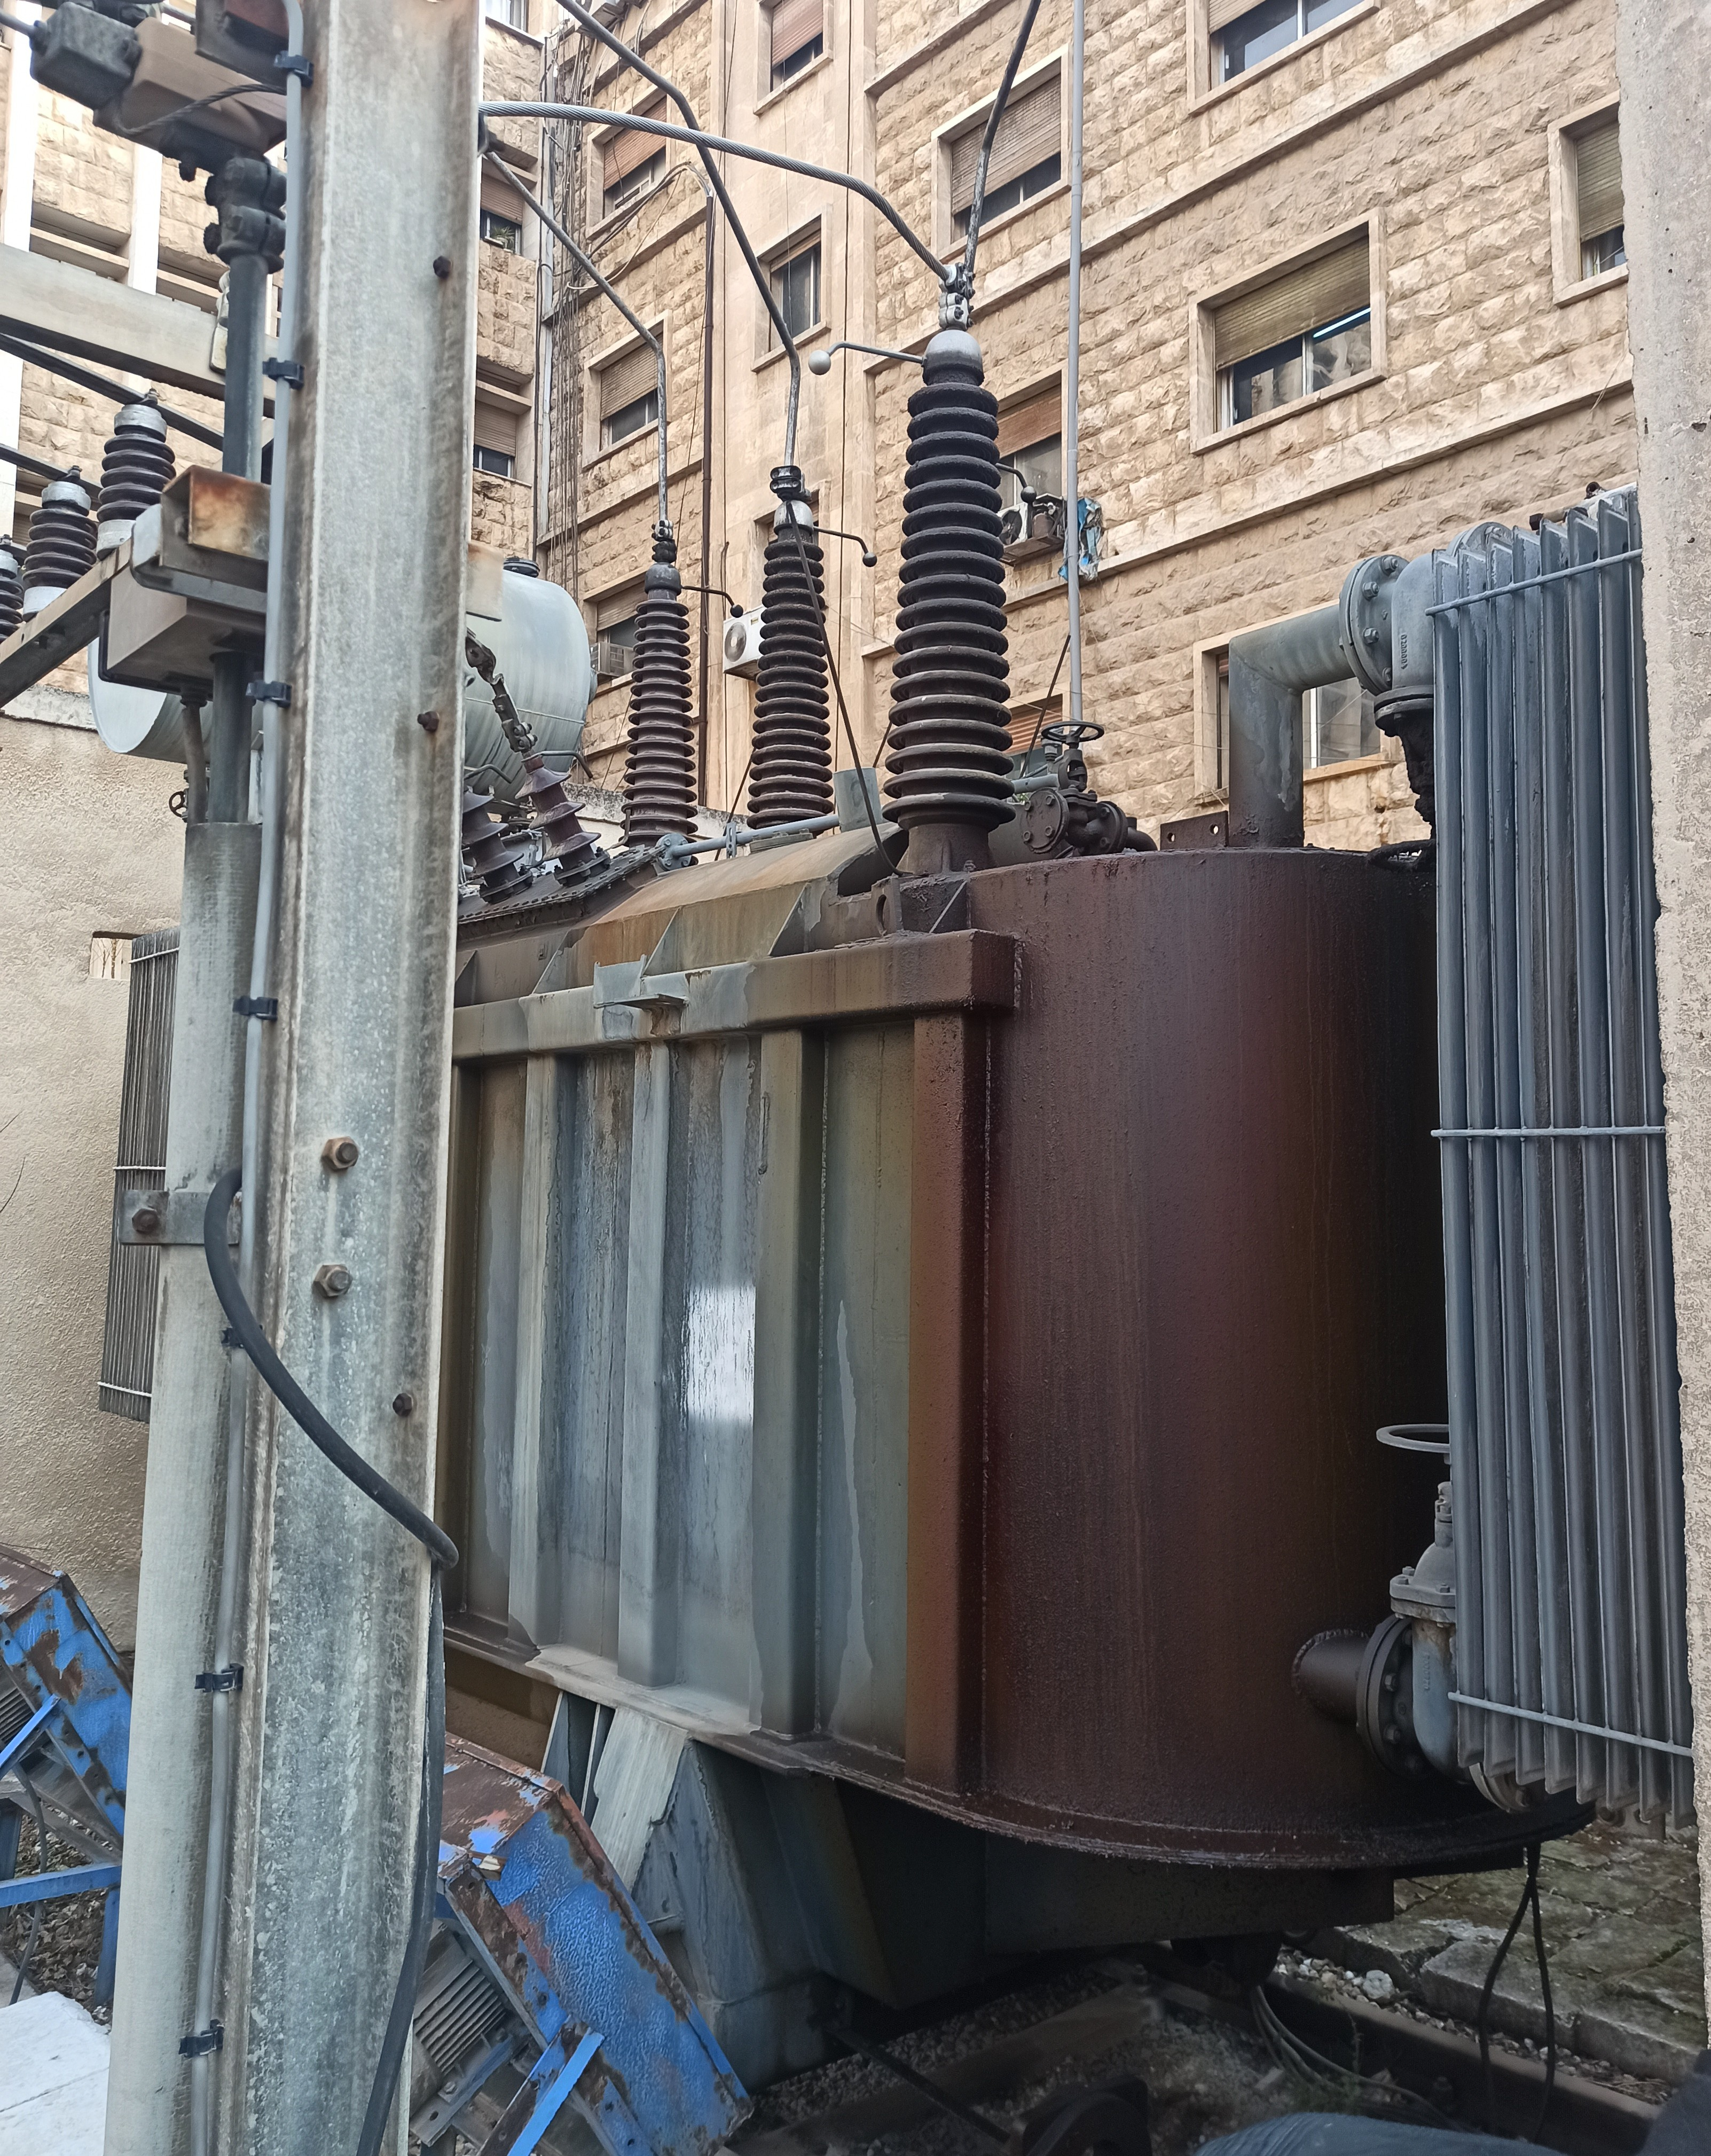
\includegraphics[width=4.5cm, height=3.5cm]{Ph0.jpg}\\
      {\footnotesize\scriptsize محول رئيسي}    
    \end{column}
  \end{columns}
    % \end{block}
  \textbf{نظام العزل والتزييت: }\fontsize{9pt}{11pt}\selectfont
  يحتوي المحول على كميات ضخمة من \textbf{زيت العزل المعدني}، وهو زيت خاص يختلف تماماً عن الزيوت العادية.\\
\end{frame}

\begin{frame}{المحول الرئيسي (القلب النابض)}
  \begin{columns}
    \begin{column}{0.45\textwidth}
      \textbf{نظام التبريد :}\\
      تعتمد المحطة على التبريد \textbf{بالتبادل الحراري} عبر "الرادياتيرات".\\
      يتم تعزيز التبريد بواسطة \textbf{مراوح كهربائية} تعمل آلياً حسب درجة الحرارة، وقد تُستخدم رشاشات المياه في الحالات القصوى للحفاظ على استقرار الاستطاعة.\\
    \end{column}
    \vspace{0.5cm}
    \begin{column}{0.45\textwidth}
      \centering
      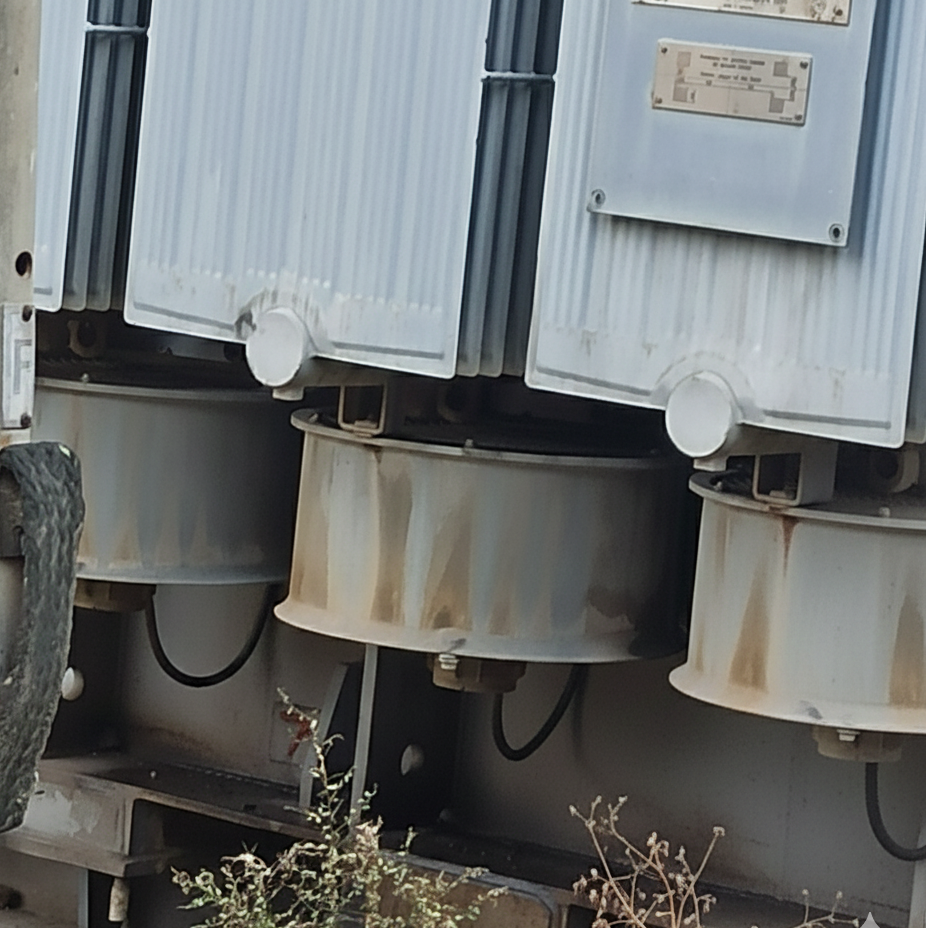
\includegraphics[width=0.9\textwidth]{Ph8.png}\\
      {\footnotesize\scriptsize مروح من بنية المحول}
    \end{column}
  \end{columns}
\end{frame}



\begin{frame}{أنظمة حماية المحول (الميكانيكية والغازية)}
  \fontsize{10pt}{12pt}\selectfont
   \textbf{حماية البوخلز :}\\
تعتبر "خط الدفاع الأول" ضد الأعطال الداخلية؛ وهي جهاز ميكانيكي غازي يركب على الأنبوب الواصل بين الخزان الرئيسي وخزان التمدد (الاحتياطي).
آلية العمل: تحتوي على "فواشات" تعطي أمر فصل للمحول في حالتين:
\begin{itemize}
  \item تولد غازات: نتيجة حدوث قصر بين الملفات يؤدي لغليان الزيت وتبخره.
  \item نقص مستوى الزيت: إذا انخفض مستوى الزيت دون حد الأمان.
\end{itemize}
\vspace{10pt}
\begin{columns}
  \begin{column}{0.55\textwidth}
    \textbf{خزان الزيت الاحتياطي :}\\
    يوجد خزان علوي يحافظ دائماً على مستوى زيت (بحدود الثلث أو الوسط) لتعويض تمدد الزيت عند الحرارة وتقلصه عند البرودة.\\
    ينقسم الخزان أحياناً إلى حجرتين؛ واحدة للمحول الرئيسي والأخرى لمنظم الجهد لضمان استقلالية الزيت في كل منهما.
  \end{column}

  \hspace{-0.8cm}

  \begin{column}{0.45\textwidth}
    \centering
    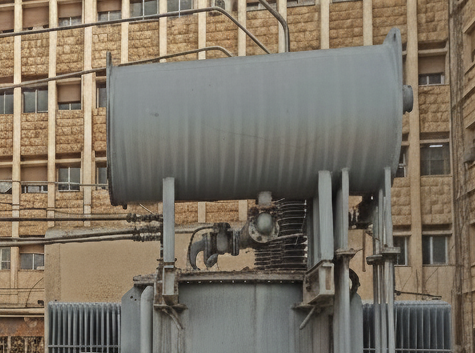
\includegraphics[width=4.8cm, height=3.6cm]{Ph7.png}\\
    {\footnotesize\scriptsize خزان الزيت الاحتياطي}    
  \end{column}
\end{columns}
\end{frame}

\begin{frame}{أنظمة حماية المحول (الميكانيكية والغازية)}
  \fontsize{10pt}{12pt}\selectfont
  \begin{columns}
    \begin{column}{0.55\textwidth}
      \textbf{مجفف الهواء :}\\[5pt]
      نظراً لتمدد وتقلص الزيت حسب الحمل، يحتاج المحول "للتنفس"؛ وهنا تبرز أهمية "السيلكا جيل" التي تقوم بسحب الرطوبة من الهواء الداخل للمحول لضمان بقاء الزيت جافاً تماماً.\\
      المراقبة: يتغير لون الحبيبات (من الأبيض أو الزهري إلى الأزرق أو الأسود) عندما تتشبع بالرطوبة، مما يستوجب استبدالها أو تجفيفها (تحميصها).\\
    \end{column}
    \hspace{-0.6cm}
    \begin{column}{0.4\textwidth}
      \centering
      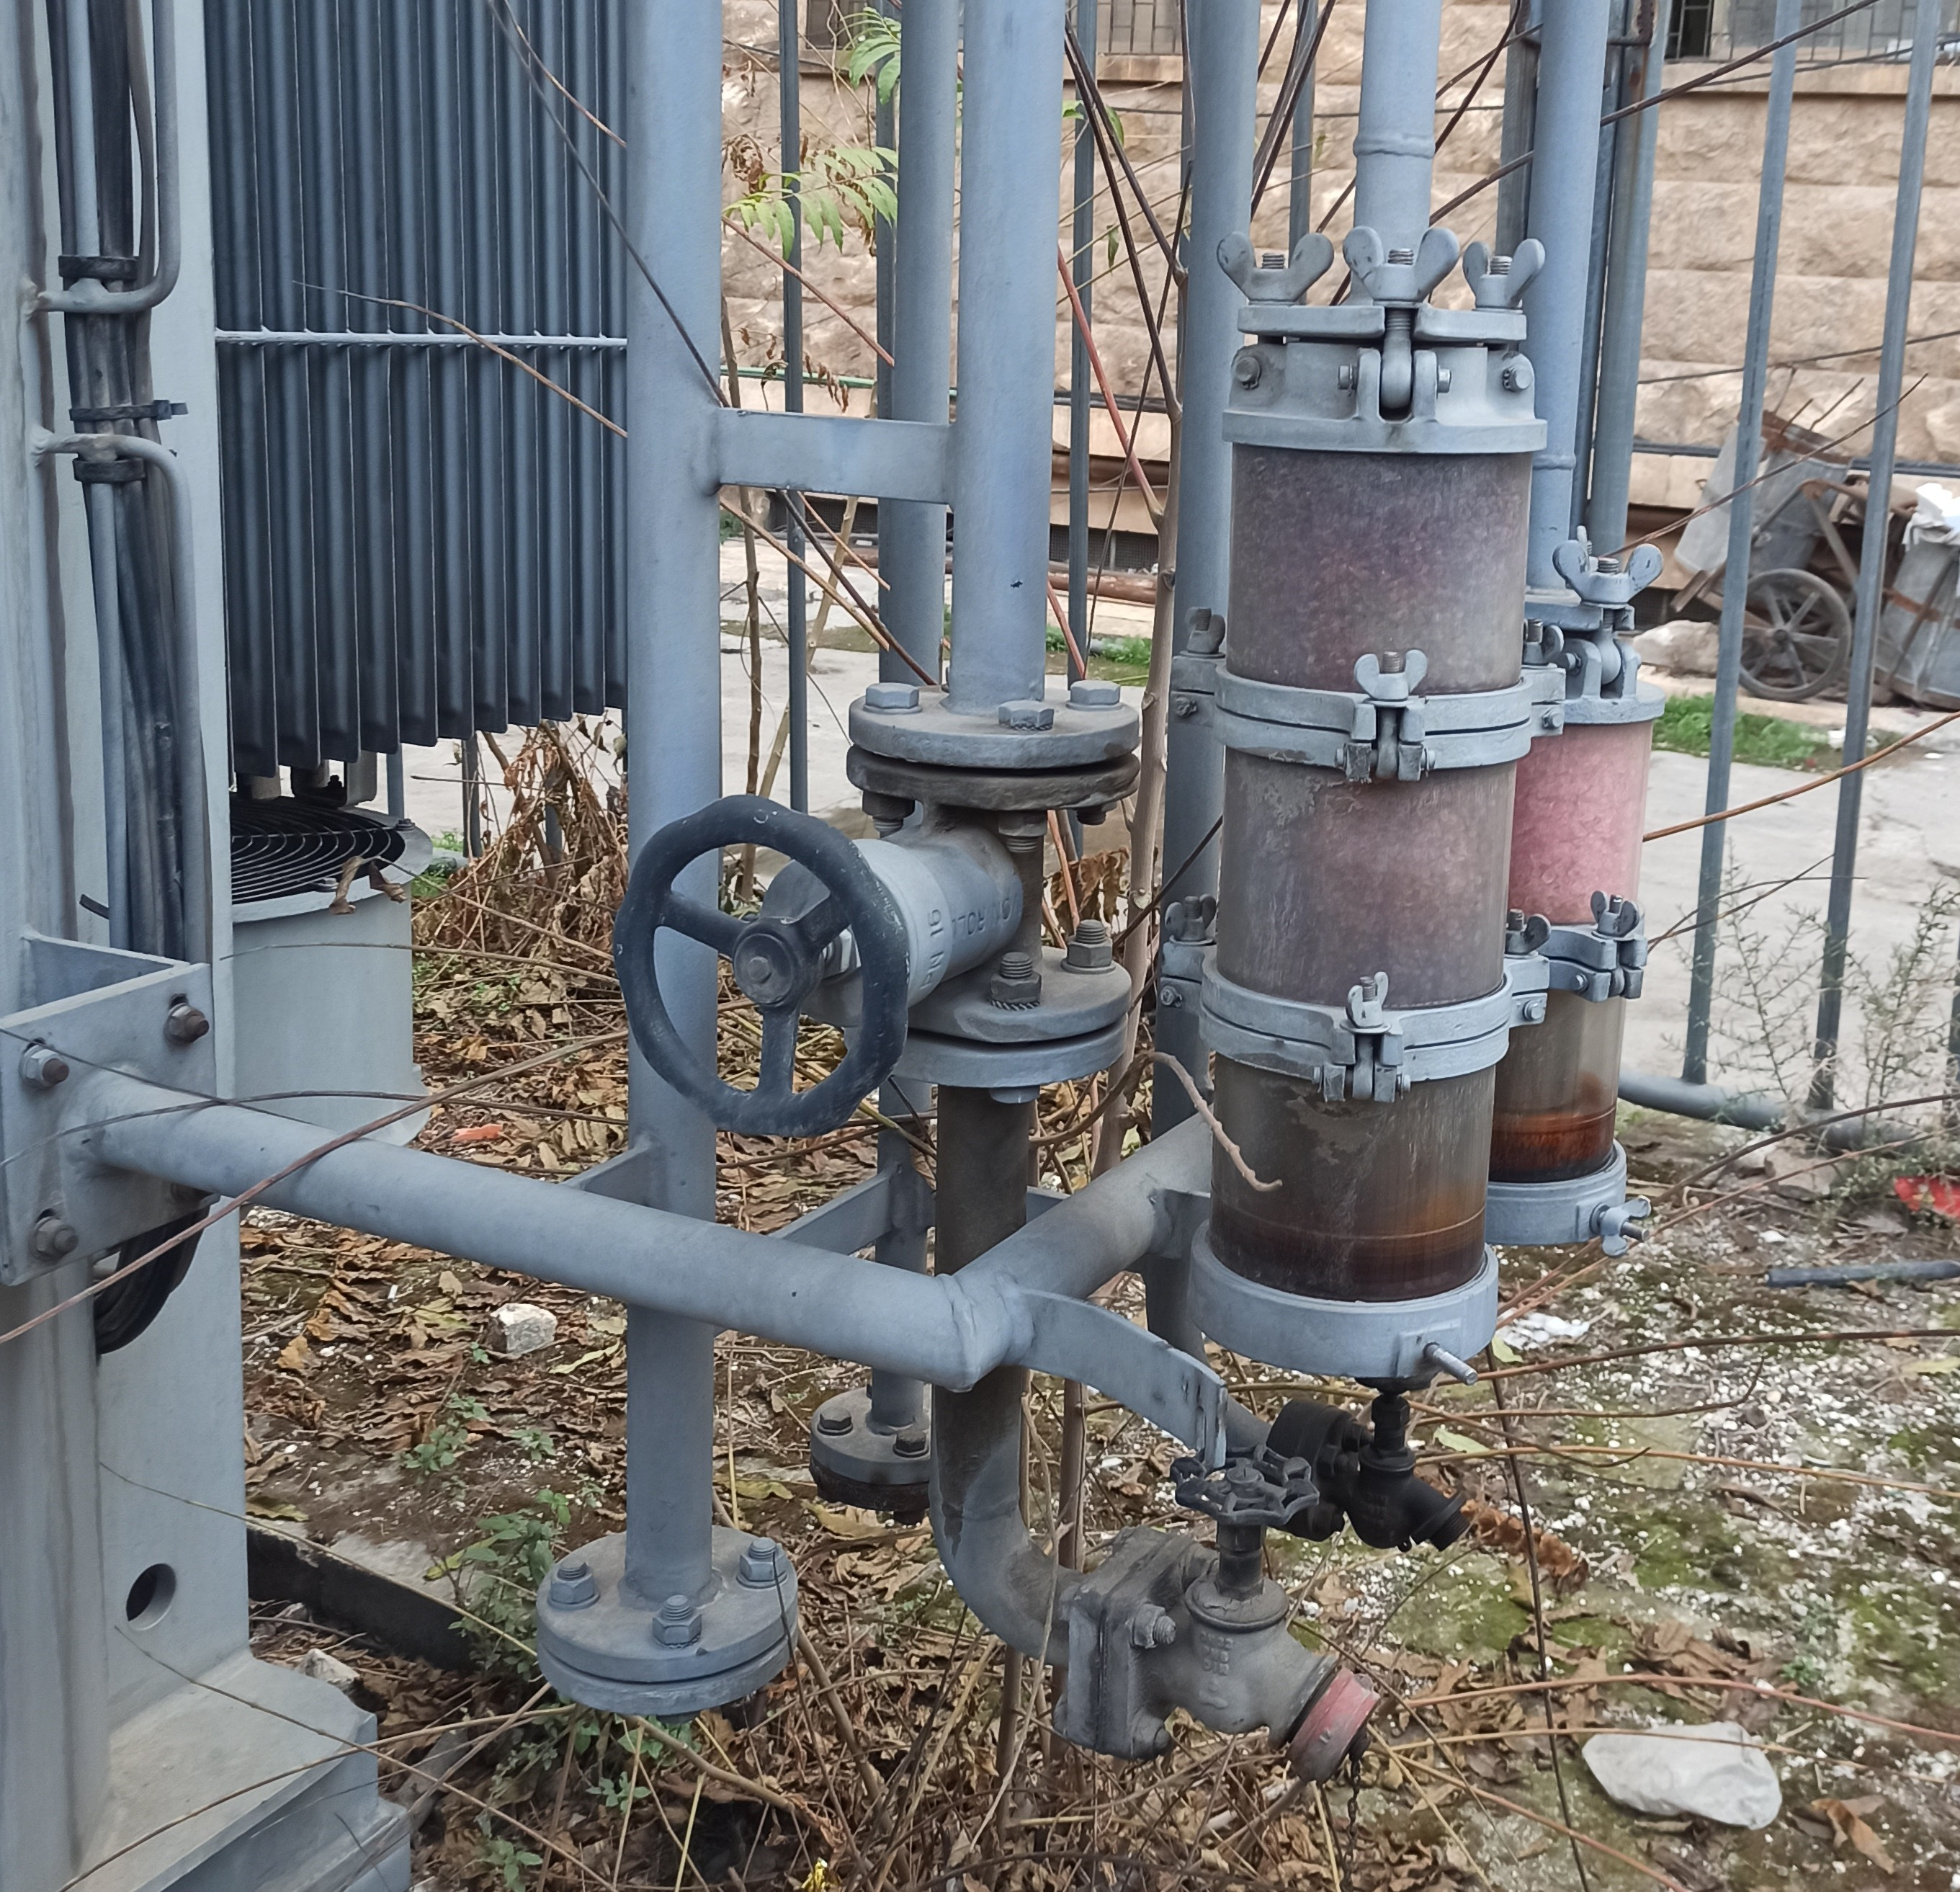
\includegraphics[width=1.1\textwidth]{Ph12.jpg}
      {\footnotesize\scriptsize مجفف الهواء }
    \end{column}
  \end{columns}
  \textbf{صمام الضغط الزائد :}\\
    يعمل تماماً مثل "صمام طنجرة الضغط"؛ ففي حال حدوث عطل انفجاري مفاجئ يولد ضغطاً هائلاً، يفتح الصمام لتفريغ الضغط وحماية جسم المحول من الانفجار الكامل.
\end{frame}

\begin{frame}{منظم الجهد تحت الحمل }
  % \metroset{block=fill}
  % \begin{block}{مفهوم التنظيم تحت الحمل \en{(On-Load)}:}
      \vspace{6pt}
    \begin{columns}
      \begin{column}{0.5\textwidth}
         يتميز هذا المنظم بقدرته على تغيير نسبة التحويل دون الحاجة لفصل التيار الكهربائي عن المشتركين، وهو ما يجعله مختلفاً عن محولات التوزيع الصغيرة ($20/0.4$ ك.ف) التي تتطلب فصلاً كاملاً للمحول عند تغيير الوضعيات.
      \end{column}
      \hspace{-1.6cm}
      \begin{column}{0.4\textwidth}
        \centering
        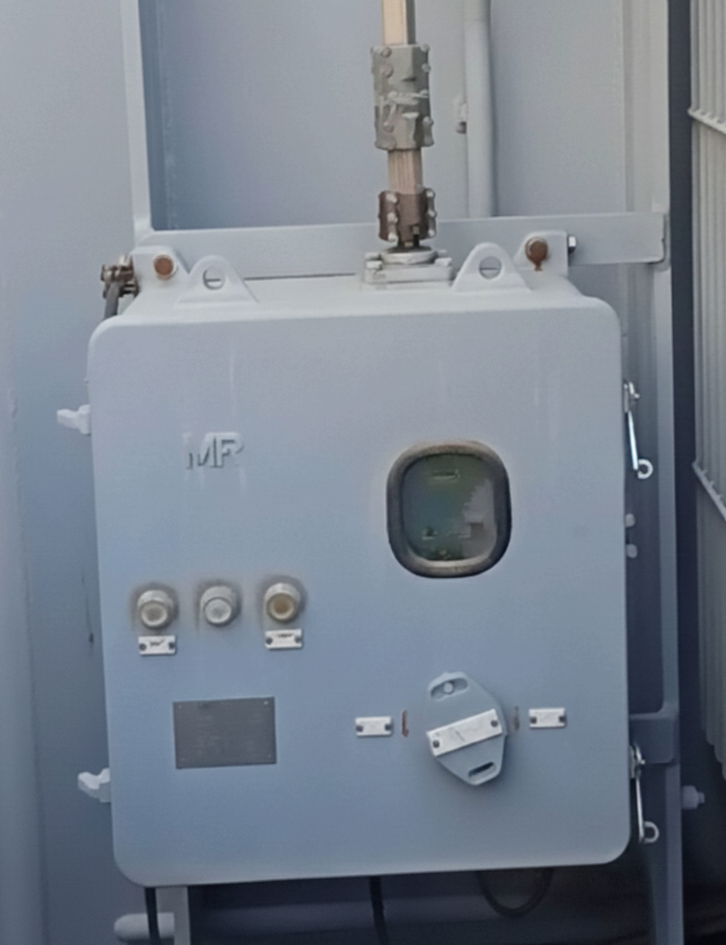
\includegraphics[width=3.2cm, height=3.8cm]{Ph13.png}\\
        {\footnotesize\scriptsize الشكل الخارجي لمنظم الجهد تحت الحمل }
      \end{column}
    \end{columns}
  % \end{block}
    \fontsize{10pt}{11pt}\selectfont
  \textbf{آلية العمل الكهربائية:}
يقوم المنظم بزيادة أو إنقاص \textbf{عدد لفات الملف الأولي (الجهد العالي)} للتحكم في قيمة الجهد الخارج من الملف الثانوي.\\
ملاحظة : يتم التغيير على جهة الجهد العالي لأن شدة التيار تكون أقل، مما يقلل من تشكل الشرارة الكهربائية أثناء عملية الانتقال بين الوضعيات.\\
\end{frame}

\begin{frame}{منظم الجهد تحت الحمل}
  \textbf{\large المكونات الميكانيكية والتشغيل:}
      \begin{itemize}
        \item \textbf{عدد الوضعيات:} يحتوي المنظم على \en{19} وضعية  تتيح رفع أو خفض الجهد بدقة عالية.\\[15pt]
        \item \textbf{محرك القيادة:} يتم التحكم في حركة المنظم بواسطة محرك كهربائي مرتبط بعلبة قيادة ميكانيكية، ويمكن تحريكه يميناً أو شمالاً (رفع/خفض).\\
      \end{itemize}
\end{frame}

\begin{frame}{منظم الجهد تحت الحمل}
  \begin{itemize}
    \item \textbf{الجزء المتحرك :} هو الجزء الداخلي الذي يقوم فعلياً بعملية التبديل بين مخارج ملفات التنظيم المجهزة مسبقاً داخل المحول.\\[10pt]
    \item \textbf{نظام الزيت المستقل:} يمتلك المنظم خزان زيت مستقل (أو حجرة معزولة في خزان التمدد) لا يختلط بزيت المحول الرئيسي؛ وذلك لأن عملية التبديل تولد شرارات كربونية تلوث الزيت، مما يتطلب استبداله أو تكريره بشكل منفصل بناءً على عدد مرات التشغيل.\\[10pt]
    \item \textbf{عداد العمليات:} يوجد عداد يسجل عدد مرات اشتغال المنظم، وهو مؤشر أساسي لتحديد مواعيد الصيانة الدورية.
  \end{itemize}
\end{frame}

\begin{frame}{نظام التأريض ومحول الخدمات }
\begin{columns}
  \begin{column}{0.45\textwidth}
    بما أن الملف الثانوي للمحول الرئيسي موصول على شكل مثلثي، فإنه يفتقر لـ نقطة حيادي تكتمل عبرها الدارة عند حدوث قصر، لذا يتم استخدام \textbf{محول تأريض مساعد} لخلق نقطة حيادي، وبهذا الطريقة تتمكن الحمايات من كشف التسريب وفصل المحول في حينها.\\
    يُستفاد من هذا المحول أيضاً في تغذية خدمات المحطة بالطاقة الكهربائية.
  \end{column}
  \hspace{-1cm}
  \begin{column}{0.45\textwidth}
    \centering
    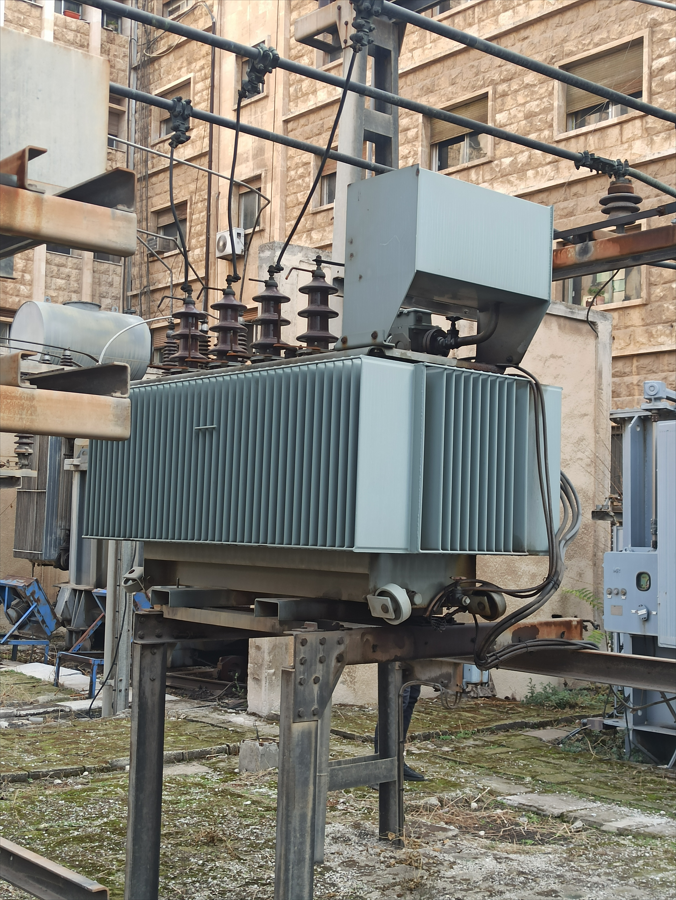
\includegraphics[width=1.1\textwidth]{Ph15.png}
  \end{column}
\end{columns}
\end{frame}

\begin{frame}{ غرفة التحكم ونظام الـ \en{DC}}
% \begin{columns}
%   \begin{column}{0.45\textwidth}
    تضم الغرفة لوحات لمراقبة الأحمال اللحظية (عبر 3 مقاييس تيار للفازات R, S, T) ومقاييس الجهد، بالإضافة لعدادات الطاقة الفعلية والردية.\\
كما يعد نظام التيار المستمر "العصب الرئيسي" للمحطة؛ فهو المسؤول عن تغذية دوائر التحكم والحماية، ولا يمكن تشغيل المحطة أو فصل القواطع بدونه، حيث يعتمد النظام على بطاريات "كاديوم" لضمان استمرار الحماية حتى عند انقطاع التغذية الكامل.\\[10pt]
  % \end{column}
  % \hspace{-1cm}
  % \begin{column}{0.45\textwidth}
    \centering
    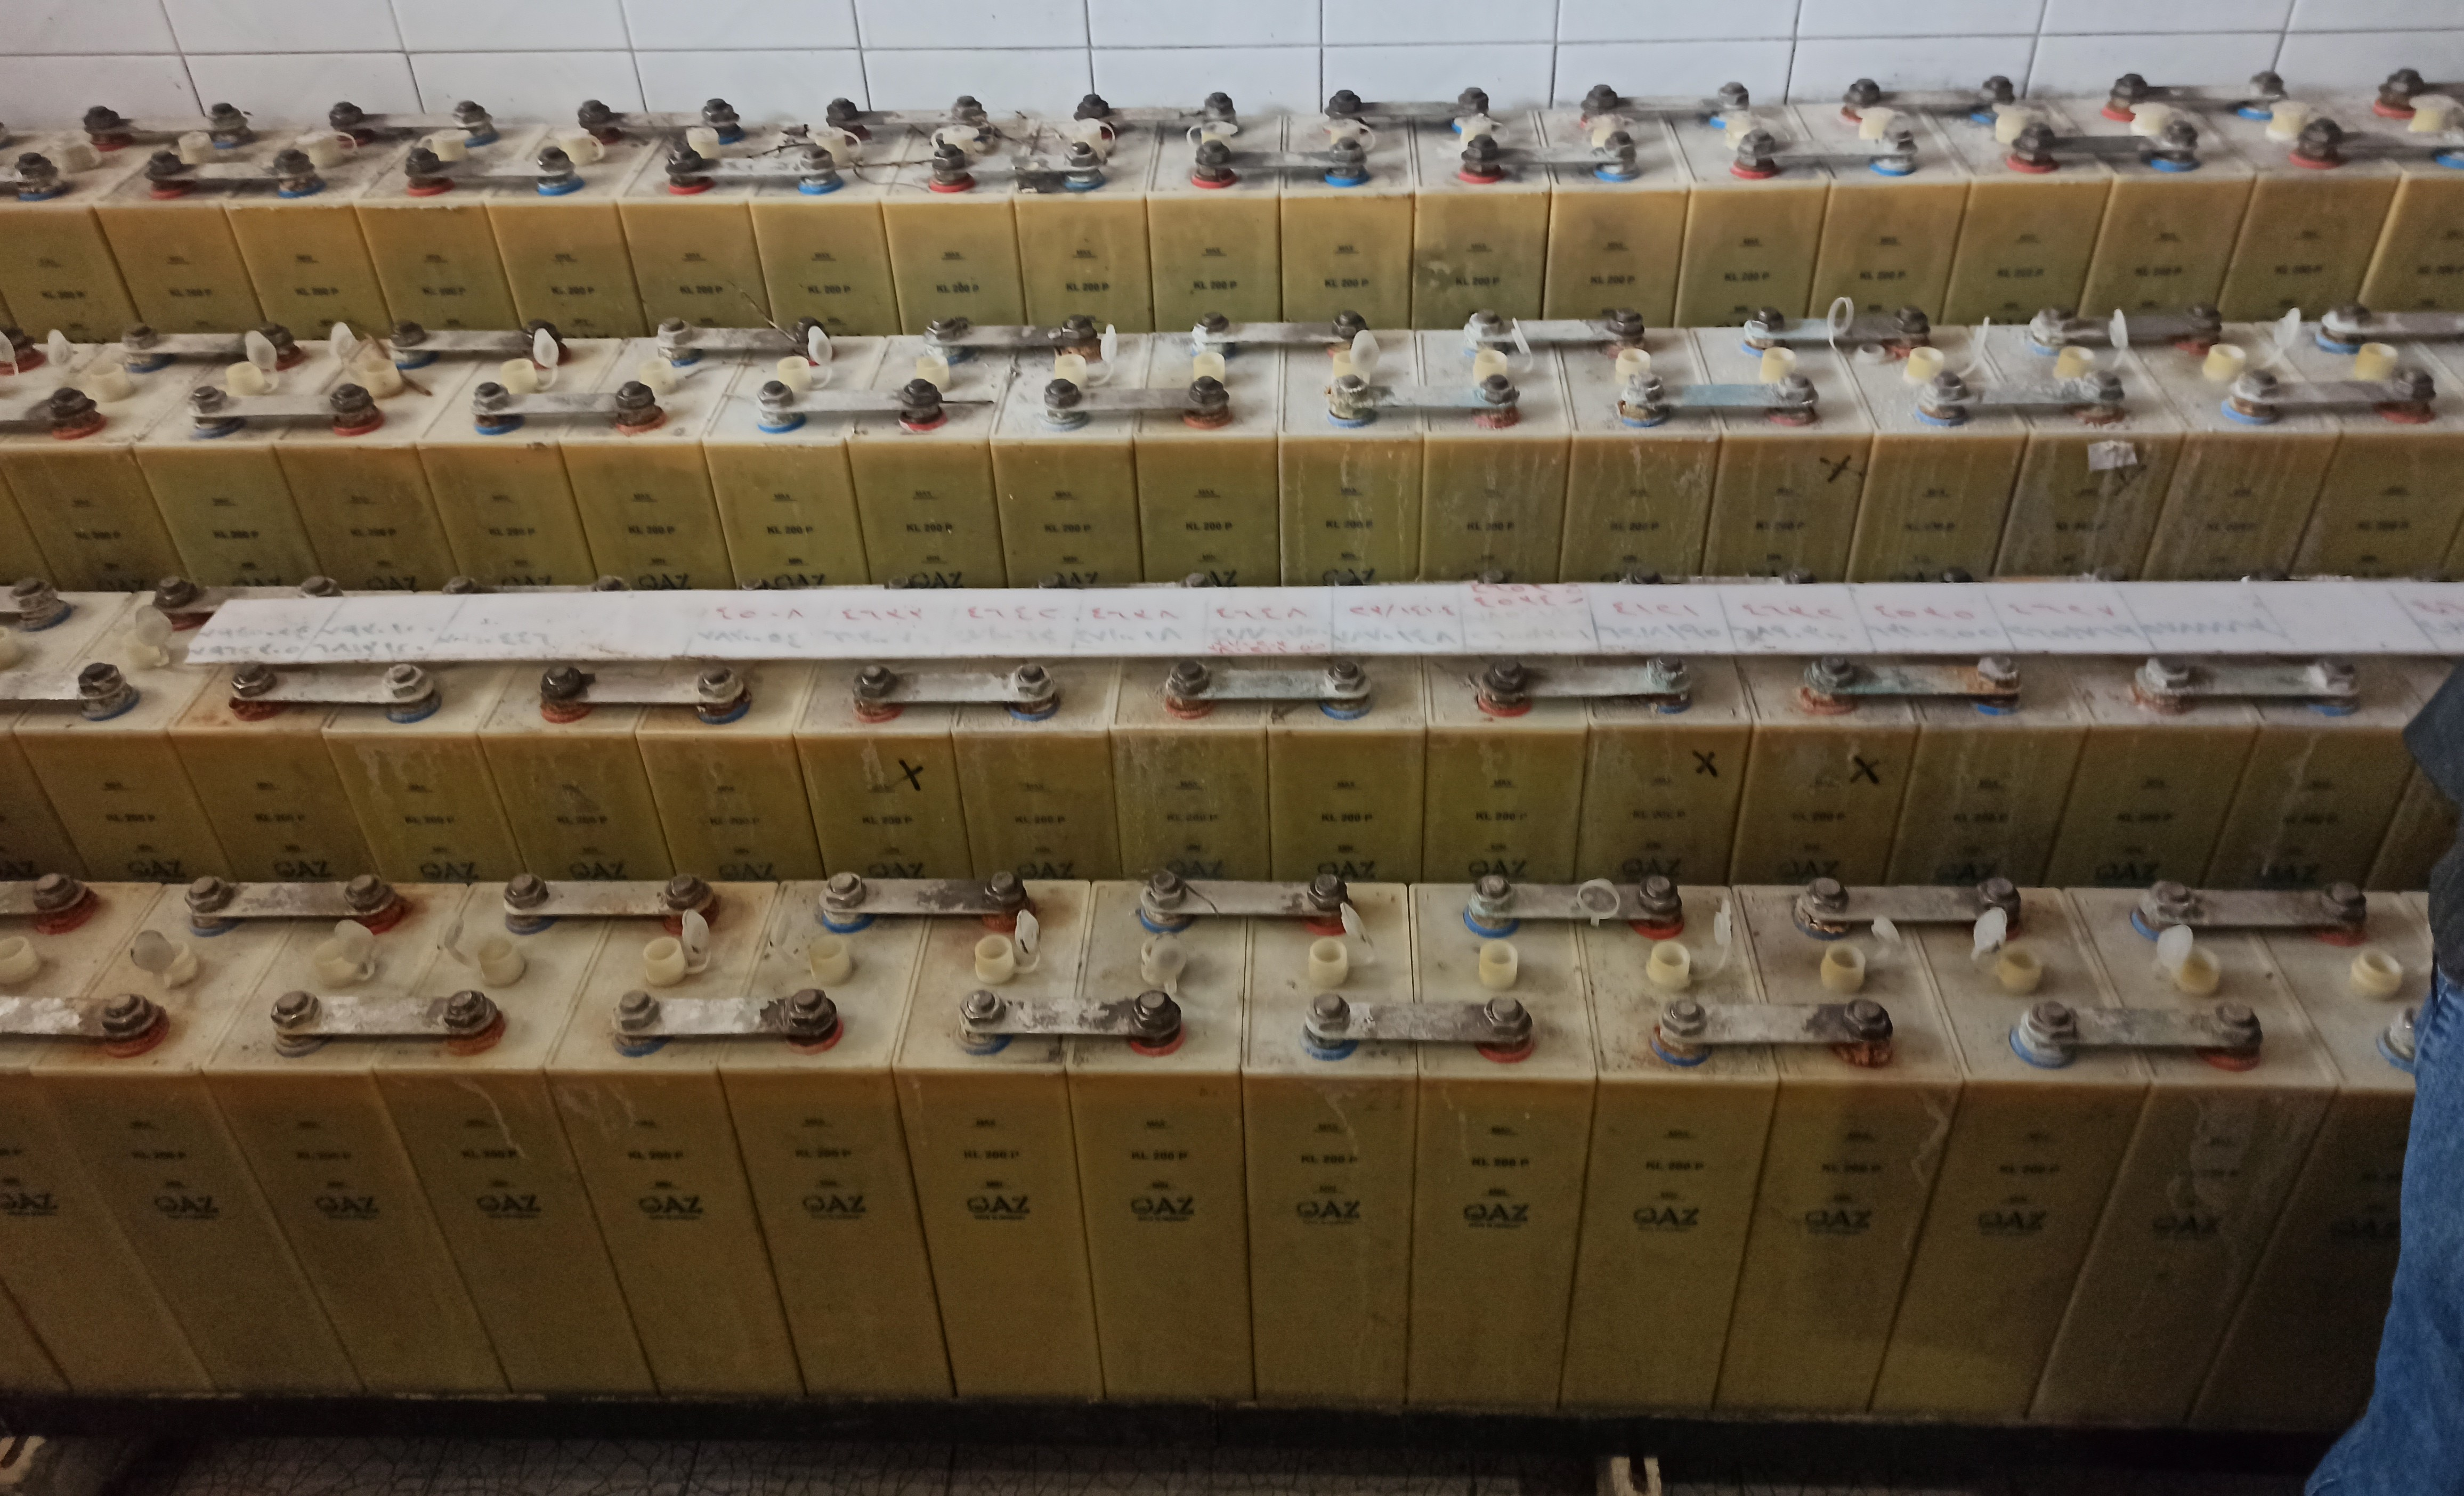
\includegraphics[width=0.7\textwidth]{Ph16.jpg}
%   \end{column}
% \end{columns}
\end{frame}

\begin{frame}{  وتوزيع الأحمال }
    يتم تقسيم المخارج حسب طبيعة المنطقة وأهميتها، بحيث لا تتجاوز استطاعة المحول؛ (مثلاً محول الـ \en{20 MVA} يتحمل حتى \en{650} أمبير).\\
  \textbf{\small عملية الكوبلاج :} هي عملية ربط البارات لضمان استمرار التغذية عند خروج محول للصيانة، أو لـ موازنة الأحمال بين المحولات.\\
  لا يمكن إتمام الكوبلاج إلا بتحقيق "التوافق" في ثلاثة شروط: تساوي التوتر، توافق التردد، وتطابق فرق الصفحة.
  
\end{frame}

% \begin{frame}[standout]
%   ختامًا نتقدم بالشكر للمهندسين والمشرفين في محطة التحويل على شروحاتهم القيمة، وللدكتور خالد حمود على إتاحة هذه الفرصة التعليمية العملية.
% \end{frame}

\end{document}